
\section{\DSU}
\ShowTOC[currentsection]
\subsection{Developer's view}

\begin{frame}{Developer's view of \DSU{}}%{A Sub-title is optional}
\begin{center}
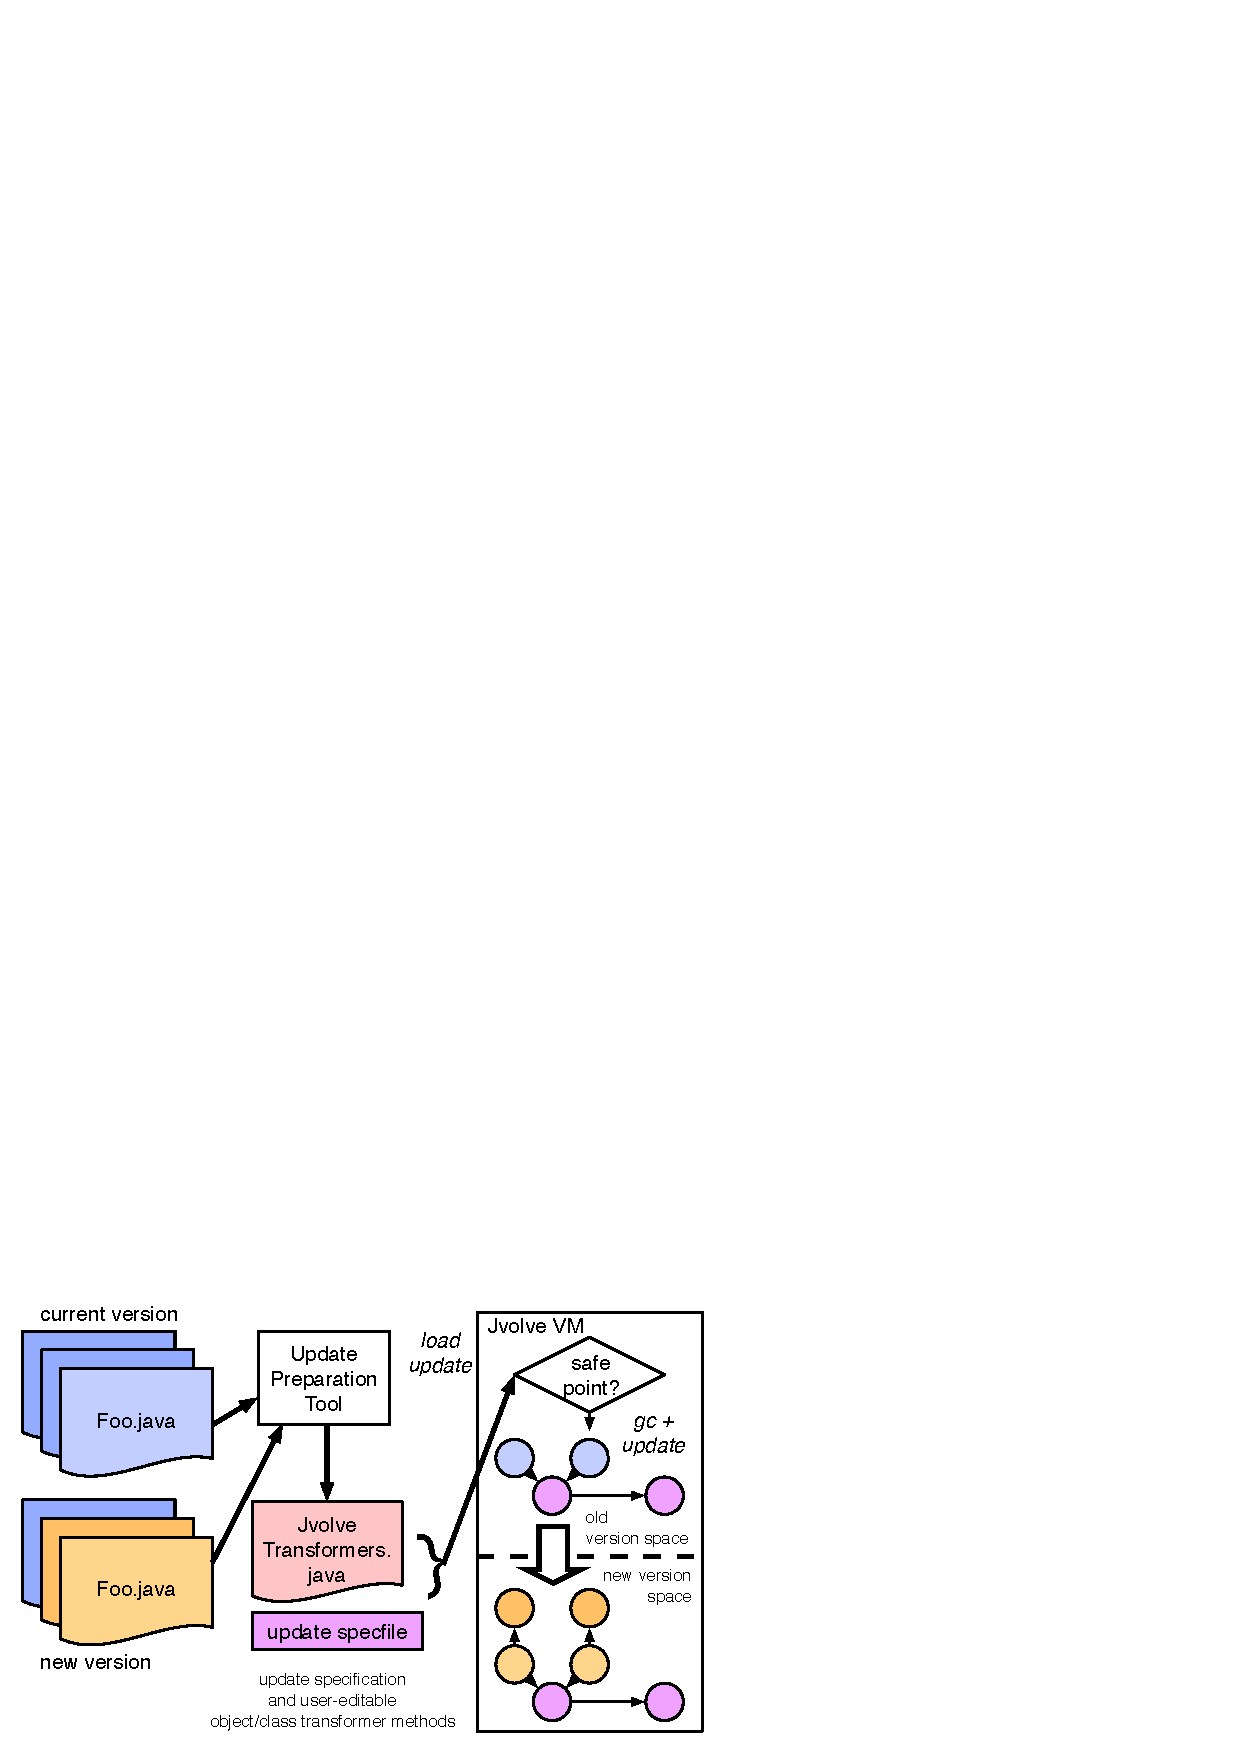
\includegraphics[width=0.84\paperwidth]{system.pdf}
\end{center}
\end{frame}

\begin{frame}{Division of Labor}%{A Sub-title is optional}
\begin{itemize}
\item Developer
  \begin{itemize}
  \item Write the old and new versions
  \item Write class/object transformation functions for classes that
        changed (optional)
  \item Testing (both the application and the update)
  \end{itemize}
\item \DSU{} system
  \begin{itemize}
  \item Update Preparation Tool (UPT) compares versions and presents the
        update to the \DSU{} VM.
  \item \DSU{} VM handles the update
  \end{itemize}
\end{itemize}
\end{frame}

\begin{frame}{Supported updates}%{A Sub-title is optional}
\begin{itemize}
\item Changes within the body of a method
\item Class signature updates
  \begin{itemize}
  \item Add, remove, change the type signature of fields and methods
  \end{itemize}
\item Changes can occur at any level of the class hierarchy
\end{itemize}
\end{frame}

\newcommand{\ExampleCodeSize}{footnotesize}
\begin{frame}[fragile,shrink=5]{Example of an update (JavaEmailServer)}%{A Sub-title is optional}
\begin{\ExampleCodeSize}
\begin{verbatim}
  public class User {
    private String username, domain, password;
    private String[] forwardAddresses;
    public String[] getForwardedAddresses() {...}
    public void setForwardedAddresses(String[] f) {...}
  }

  public class ConfigurationManager {
    private User loadUser(...) {
       ...
       User user = new User(...);
       String[] f = ...;
       user.setForwardedAddresses(f);
       return user;
    }
  }




\end{verbatim}
\end{\ExampleCodeSize}
\end{frame}

% \begin{frame}[fragile,shrink=5]{Example of an update (JavaEmailServer)}%{A Sub-title is optional}
% \begin{\ExampleCodeSize}
% \begin{semiverbatim}
% public class User \{
%   private String username, domain, password;
%   private \sout{String[]} EmailAddress[] forwardAddresses;
%   public \sout{String[]} EmailAddress[] getForwardedAddresses() \{...\}
%   public void setForwardedAddresses(\sout{String[]} EmailAddress[] f) \{...\}
% \}
% 
% public class ConfigurationManager \{
%   private User loadUser(...) \{
%      ...
%      User user = new User(...);
%      \sout{String[]} EmailAddress[] f = ...;
%      user.setForwardedAddresses(f);
%      return user;
%   \}
% \}
% 
% \end{semiverbatim}
% \end{\ExampleCodeSize}
% \end{frame}

\begin{frame}[fragile,shrink=5]{Example of an update (JavaEmailServer)}%{A Sub-title is optional}
\newcommand{\removed}[1]{\textcolor{red}{- #1}}
\newcommand{\addedxx}[1]{\textcolor{OliveGreen}{+ #1}}
\begin{\ExampleCodeSize}
\begin{semiverbatim}
  public class User \{
    private String username, domain, password;
\removed{  private String[] forwardAddresses;}
\removed{  public String[] getForwardedAddresses() \{...\}}
\removed{  public void setForwardedAddresses(String[] f) \{...\}}
\addedxx{  private EmailAddress[] forwardAddresses;}
\addedxx{  public EmailAddress[] getForwardedAddresses() \{...\}}
\addedxx{  public void setForwardedAddresses(EmailAddress[] f) \{...\}}
  \}

  public class ConfigurationManager \{
    private User loadUser(...) \{
       ...
       User user = new User(...);
\removed{     String[] f = ...;}
\addedxx{     EmailAddress[] f = ...;}
       user.setForwardedAddresses(f);
       return user;
    \}
  \}
\end{semiverbatim}
\end{\ExampleCodeSize}
\end{frame}

\begin{frame}{Object Transformers}%{A Sub-title is optional}
\begin{itemize}
\item ``Transform'' objects to correspond to the new version
\item A function specified as part of the new version of a class
\item Accepts old object and new object as parameters
\item VM runs a default transformer that copies old fields and initializes
new ones to \texttt{null}
\end{itemize}
\end{frame}

\begin{frame}[fragile,shrink=5]{Object Transformers}%{A Sub-title is optional}
\mode<beamer> {
\begin{textblock*}{46mm}[0,0](79mm,20mm)
\begin{block}{}
Stub generated by UPT for the old version
\end{block}
\end{textblock*}
\begin{textblock*}{46mm}[0,0](79mm,48mm)
\begin{block}{}
Default transformer copies old fields, initializes new ones to
\texttt{null}
\end{block}
\end{textblock*}
}
\begin{small}
\begin{semiverbatim}
public class old_User \{
  public String username, domain, password;
  public String[] forwardAddresses;
\}
public class User \{
  ...
  public static void jvolve_class() \{ ... \}
  public static void jvolve_object(User to, old_User from) \{
    to.username = from.username;
    to.domain = from.domain;
    to.password = from.password;
    to.forwardAddresses = null;
    \uncover<2>{int l = from.forwardAddresses.length;
    to.forwardAddresses = new EmailAddress[l];
    for (int i = 0; i < l; i++)
      to.forwardAddresses[i] =
       new EmailAddress(from.forwardAddresses[i]);
}\}\}

\end{semiverbatim}
\end{small}
\end{frame}
